\documentclass{article}

\usepackage{float}
\usepackage{xepersian}

\settextfont{XB Zar}

\title{اسامی گروه و موضوع پروژه}

\date{}

\begin{document}

\maketitle

\section*{اعضای گروه}
\vspace{0.5cm}

\begin{itemize}

\item \textbf{محمدحسین اعلمی \hspace{0.5cm} ۹۴۱۰۴۴۰۱}
\item \textbf{علی عسگری \hspace{1.4cm} ۹۴۱۰۵۳۷۷}

\end{itemize}

\section*{موضوع پروژه:‌ دستیار برنامه ریزی}

پایگاه داده ای برای برنامه ای کاربردی پیاده سازی خواهیم کرد که دستیاری برای مدیریت و برنامه ریزی امور
\footnote{\lr{task management}}
 و تحلیل زمان صرف شده برای کارهای مختلف است. در این سیستم کاربر قابلیت این را دارد که وظیفه‌هایی تعریف کرده، برای آن وظیفه‌‌ها زمان انجام شدن، یادآور، توضیحات و زیروظیفه‌هایی برای آن تعریف کند. هم‌چنین می‌توان وظیفه‌ها را در فهرست‌ها و دسته‌بندی‌های منحصر به فرد قرار داد و فهرست‌ها را با دیگر کاربران به اشتراک گذاشت. هم‌چنین قابلیت عملیات‌ آماری بر روی زمانهای درنظرگرفته‌شده و زمان واقعی انجام وظیفه‌ها وجود دارد. این برنامه‌ مشابه برنامه کاربردی Wunderlist با قابلیت‌ها و امکانات بیشتر است.
 
\section*{نیازمندی‌ها}	

برخی از موجودیت‌های سیستم به شرح زیر است:

\begin{itemize}

\item در این محیط تعدادی کاربر داریم که اطلاعات آن‌ها مانند رایانامه، نام‌ کاربری، اطلاعات ورود به حساب و عکس موجود است.

\item در این محیط تعدادی وظیفه
\footnote{\lr{task}}
 تعریف می‌شود که هر وظیفه شامل ویژگی‌هایی مانند نام، زمان و مهلت اجرا، زمان پیش‌بینی‌شده و واقعی اجرا، تکرار شوندگی، برچسب‌ها، توضیحات و ... است. هم چنین هر وظیفه تعدادی زیر‌‌وظیفه نیز دارد.
 
 \item زیروظیفه‌هایی داریم که به نوعی کار‌های مربوط به یک وظیفه هستند و شامل نام و وضعیت انجام(انجام شده یا نشده) هستند.
 
 \item می‌توان برای هر وظیفه‌ یادآور‌هایی با زمان، تکرار‌شوندگی و روش ارسال مشخص نیز تنظیم کرد.
 
 \item فهرست‌هایی داریم که دارای یک نام مشخص و تعدادی وظیفه است. هم‌چنین فهرست‌های اشتراکی نیز داریم که در آن یک یا چند کاربر مدیر هستند و می‌توانند وظیفه‌ها را به دیگر کاربر‌های عضو فهرست منتسب کنند.
 
\item پوشه‌هایی داریم که می‌توان فهرست‌های مرتبط را درون یکی از آن‌ها قرار داد. هر فهرست یک نام دارد.

\item
می توان کاربران مدیر سیستم را هم به عنوان یک موجودیت در نظر گرفت.

\end{itemize}

نیازمندی‌های کاربردی سیستم نیز به صورت زیر است:

\begin{itemize}

\item کاربر می‌تواند در سیستم ثبت‌نام کرده و اطلاعات خود را ویرایش کند

\item کاربر می‌تواند فهرست‌هایی  با نام‌‌های مشخص ایجاد کرده و درون آن‌‌ها وظیفه‌های جدیدی تعریف کند.

\item کاربر می‌تواند در هر فهرست‌ وظیفه‌هایی با ویژگی‌های مشخص تعریف کرده و آن‌ها را ویرایش کند. پس از تایید انجام شدن یک وظیفه توسط کاربر آن وظیفه به آرشیو همان فهرست منتقل می‌شود. این آرشیو در صورت لزوم قابل مشاهده خواهد بود.

\item کاربر می‌تواند برای هر وظیفه یاد‌آور‌هایی که به صورت یک‌باره یا تکرار‌پذیر به شکل روزانه، هفتکی، ماهانه و... تعریف کند.

\item کاربر( یا کاربرها در فهرست‌های اشتراکی) می‌تواند زیر هر وظیفه‌ نظر‌اتی بگذارد.

\item کاربر یک زمان پیش‌بینی شده برای هر وظیفه تعیین می‌کند و در هنگام انجام آن وظیفه با استفاده از زمان‌سنج برنامه زمان واقعی انجام وظیفه را اندازه‌گیری می‌کند.

\item کاربر برای هر وظیفه یک مهلت نهایی و زمان انجام تعریف می‌کند که تعیین هر دوی این موارد در زمان تعریف وظابف اختیاری است.

\item کاربر می‌تواند برای هر وظیفه منابعی مانند عکس، مستند و... تعریف کند. هم‌چنین برای هر وظیفه می‌توان برچسب‌های مشخصی تعیین کرد.

\item کاربر می‌تواند فهرست‌های اشتراکی تعریف کرده و در آن‌ها کاربر‌های دیگری اضافه کند. هر فهرست اشتراکی شامل چند کاربر مدیر است که می‌توانند وظیفه‌ها را به دیگر کاربر‌ها منتسب کنند. سایر کاربر‌های نیز می‌توانند وظایف خود را ویرایش کرده و ذیل وظایف دیگر کاربر‌ها نظر بدهند.

\end{itemize}

نیاز‌مندی‌های گزارشی سیستم نیز به صورت زیر است:

\begin{itemize}

\item کاربر می‌تواند وظایف مربوط به هر پوشه و فهرست یا دارای برچسب خاصی را مشاهده کند.

\item کاربر می‌تواند نظرات اخیر بقیه کاربر‌ها را مشاهده کند.

\item کاربر می‌تواند فعالیت‌های اخیر خود و بقیه کاربر‌ها را مشاهده کند.

\item کاربر می‌تواند وظایف ضروری مربوط به یک روز، هفته، ماه یا بازه زمانی مشخصی را مشاهده کند.

\item کاربر می‌تواند وظایف را در فهرست‌ها بر اساس مهلت انجام، زمان انجام، مدت‌زمان پیش‌بنی‌شده و ضرورت مرتب‌سازی کند.

\item کاربر می‌تواند همه‌ی وظیفه‌هایی که زمان انجام آن‌ها در روز، هفته، ماه یا هر بازه‌ی زمانی مشخصی است را مشاهده کند.

\item کاربر می‌تواند وظیفه‌هایی که مهلت انجام آن‌ها تا زمان مشخصی‌ است را با تعیین کردن آن زمان مشاهده‌ کند.

\item کاربر می‌تواند هر دو ویژگی بالا را با فیلتر پوشه‌، فهرست یا برچسب انجام دهد.

\item کاربر می‌تواند مجموع زمان پیش‌بینی‌شده لازم برای یک پوشه، فهرست و یا برچسب مشخص را در هر بازه زمانی مشاهده کند.

\item کاربر می‌تواند مجموع زمان سپری‌شده(واقعی) برای انجام وظیفه‌های یک فهرست، پوشه یا برچسب را در یک بازه زمانی مشخص‌ در گذشته مشاهده کند.

\item کاربر می‌تواند با دادن مدت‌زمانی که می‌تواند در آینده نزدیک صرف انجام کاری کند طولانی‌ترین وظیفه‌ای را که مدت زمان پیش‌بینی شده آن از زمان داده‌شده کمتر است مشاهده کند.

\item کاربر می‌تواند کارکرد متوسط روزانه یا هفتگی خود را در یک بازه زمان مشخص( مثلا از ابتدا تا کنون) مشاهده کند. این مقدار از جمع ساعات واقعی وظایف آن کاربر به دست می‌آید.

\item کاربر مدیر در فهرست اشتراکی می‌تواند مجموع زمان آزاد هر کاربر در آینده را مشاهده کند. به این صورت که یک بازه زمانی از آینده مشخص می‌شود و مجموع زمان پیش‌بینی شده برای انجام وظایف آن کاربر در آن بازه از کارکرد متوسط پیش‌بینی شده برای کاربر در آن زمان کسر می‌شود.

\item کاربر می‌تواند درصد تفاوت پیش‌بینی‌ زمان‌های مورد نیاز با زمان‌های واقعی را برای یک وظیفه یا وظایف متعلق به یک بازه زمانی خاص یا وظایف مربوط به یک پوشه، فهرست یا یک برچسب مشاهده نماید..

\item  کاربر می‌تواند مدت زمان تاخیر انجام شدن یک وظیفه یا مجموع مدت زمان تاخیر مربوط به انجام همه‌ی وظایف متعلق به یک بازه زمانی خاص یا مربوط به یک پوشه، فهرست یا برچسب خاص را مشاهده نماید.

\item طبعا ممکن است نیاز‌های گزارشی یا تحلیلی دیگری که به کاربر برای برنامه‌ریزی کمک می‌کند نیز به این فهرست اضافه شود.

\end{itemize}
نیازمندیهای مربوط به مدیر(ان) سیستم:
\begin{itemize}
	\item
	مدیر سیستم می تواند تعداد کاربرانی که در روز جاری از سیستم استفاده کرده اند را مشاهده کند
	\item
	مدیر سیستم می تواند تعداد کاربرانی که به سیستم در یک بازه زمانی اضافه شده اند را مشاهده کند
	\item
	مدیر سیستم می تواند در هر دوره زمانی درصد رشد کاربران را مشاهده کند
	\item
	مدیر می تواند موجودیتهای مختلف را از جمله کاربران، لیستها و ... را حذف کند، مثلا در سناریویی که یک سیستم اتوماتیک دارد از سیستم استفاده بیش از حد برای از دسترس خارج کردن سیستم انجام می دهد. 
	\item
	مدیر می تواند کاربران دیگری ایجاد کند که مدیر باشند یا کاربرانی را به مدیر ارتقاء دهد.  
\end{itemize}

\section*{طراحی نمودار}
نمودار پروژه با نرم افزار TerraER طراحی شد و در شکل \ref{fig:er} مشاهده است:
\begin{figure}[ht]
  \centering  
  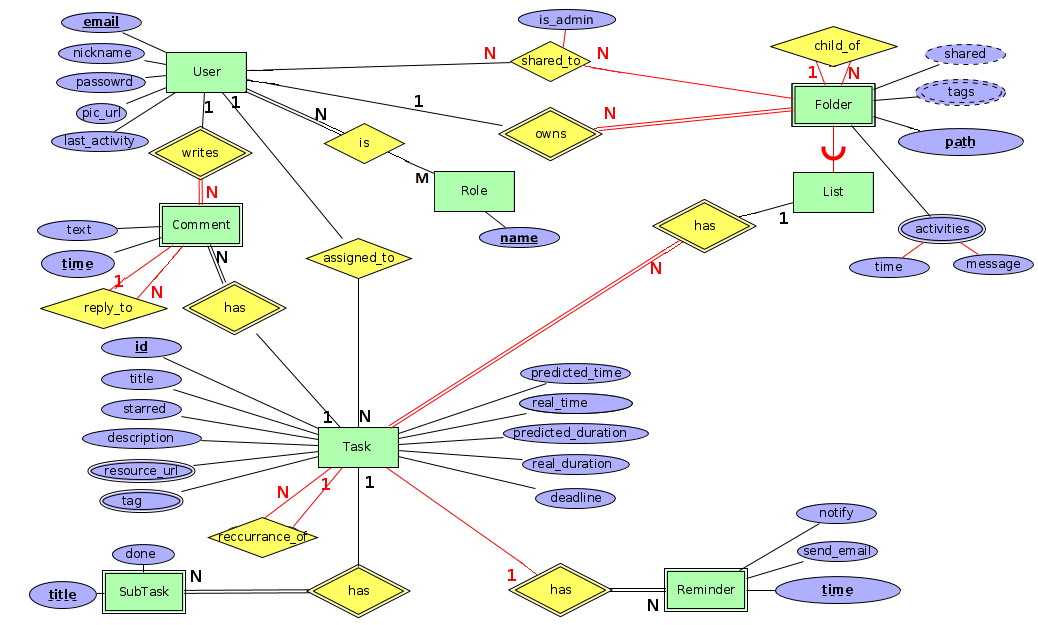
\includegraphics[width = 1\textwidth]{er.png}
  \caption{نمودار ER مربوط به پروژه}
  \label{fig:er}
\end{figure}

\section*{طراحی منطقی}
\subsection*{دامنه صفات} \label{sect:domains}
با توجه به کلیات پروژه و صفات‌ها دامنه‌ها و انواع زیر را برای پایگاه داده در نظر گرفتیم:
\begin{itemize}
	\item
	email\_domain
	: محدودیتهای استاندارد ایمیل را با استفاده از امکان عبارت منظم در postgres پیاده‌سازی کردیم. 
	\item
	label\_domain
	: این دامنه عبارت‌های کوتاه و برچسبهاست. این دامنه از جنس VARCHAR و با طول حداکثر ۳۲ تعریف می‌شود و محدودیت خاصی به جز اندازه ندارد.
	\item
	nickname\_domain
	: همان label\_domain است. 
	\item
	password\_domain
	: با توجه به این که برای گذرواژه از الگوریتم درهمسازی md5 استفاده خواهد شد، آن را از جنس CHAR  32 بیت تعیین کردیم. 
	\item
	url\_domain
	: این دامنه را از جنس VARCHAR و حداکثر به طول 512 تعیین کردیم. 
	\item
	resource\_url\_domain
	: همان url\_domain است که هیچمقدارناپذیر است. 
	\item
	pic\_url\_domain
	: همان url\_domain است با این تفاوت که هیچمقدار نا پذیر است و یک مقدار پیشفرض \LTRfootnote{	http://www.gravatar.com/avatar/00095965ca2e9b81c365d541b9cc73ec?s=40\&d=identicon
	} برای آن در نظر گرفتیم. 
	\item
	time\_setting\_domain
	: برای نگهداری داده‌های زمانی هیچ مقدار پذیر از این دامنه استفاده خواهیم کرد و جنس آن را از TIME قرار دادیم. 
	\item
	log\_time\_domain
	: برای ذخیره زمان اتفاقاتی که افتاده‌اند از قبیل زمان ارسال یک نظر و یا فعالیت از آن استفاده می‌کنیم. از جنس TIME و هیچمقدارناپذیر است. 
	\item
	text\_domain
	: برای ذخیره مقدارهای هیچمقدارپذیر متنی مانند توضیحات کارها از این دامنه استفاده کردیم. از نوع VARCHAR و به طول حداکثر 8192 است.
	\item
	comment\_text\_domain
	: برای دامنه نظرات از این دامنه استفاده خواهیم کرد که مشابه text\_domain است با این تفاوت که هیچ‌مقدارناپذیر است. 
	\item
	title\_domain
	: برای عنوانها این دامنه را در نظر گرفتیم که از نوع VARCHAR و به طول حداکثر 1024 است. عنوانها را هیچمقدارناپذیر در نظر گرفتیم. 
	\item
	boolean\_domain
	: این دامنه همان BOOLEAN سیستم مدیریت داده postgres به صورت هیچ مقدار ناپدیر است. این دامنه را برای آن لحاظ کردیم که در صورتی که در آینده و در فاز نگهداری سیستم نیاز به تغییر در کل صفات از این نوع شد بتوان یکجا تغییرات را اعمال کرد. 
	\item
	reccurrance\_id\_domain
	: این دامنه همان INTEGER سیستم مدیریت داده postgres است. این دامنه را برای آن لحاظ کردیم که در صورتی که در آینده و در فاز نگهداری سیستم نیاز به تغییر در کل صفات از این نوع شد بتوان یکجا تغییرات را اعمال کرد. 
	\item
	id\_domain
	: این دامنه همان INTEGER سیستم مدیریت داده postgres است که آن را هیچمقدارناپذیر قرار دادیم. این دامنه را برای آن لحاظ کردیم که در صورتی که در آینده و در فاز نگهداری سیستم نیاز به تغییر در کل صفات از این نوع شد بتوان یکجا تغییرات را اعمال کرد. 
	\item
	duration\_domain
	: از این دامنه برای نگهداری مدتهای زمانی استفاده کردیم و از نوع INTERVAL قرارش دادیم و فقط اجازه دادیم مقادیر مثبت داشته باشد. 
\end{itemize}
صفات طراحی اولیه رابطه‌ها در زیر آمده اند.
\latin
\begin{itemize}
\item \textbf{User}

	\begin{itemize}
	
	\item email\_domain::email
	
	\item nickname\_domain::nickname
	
	\item password\_domain::password
	
	\item pic\_url\_domain::pic\_url
	
	\item log\_time\_domain::last\_activity
	\end{itemize}
	
\item \textbf{Comment}

	\begin{itemize}
	\item comment\_text\_domain::text
	\item log\_time\_domain::time
	\end{itemize}
	
\item \textbf{Task}

	\begin{itemize}
	\item auto\_increment\_domain::id
	\item title\_domain::title
	\item boolean\_domain::starred
	\item text\_domain::description
	\item resource\_domain::resource\_url
	\item label\_domain::tag
	\item time\_setting\_domain::predicted\_time
	\item time\_setting\_domain::real\_time
	\item time\_setting\_domain::predicted\_duration
	\item time\_setting\_domain::real\_duration
	\item time\_setting\_domain::deadline
	\end{itemize}
	
\item \textbf{SubTask}

	\begin{itemize}
	\item title\_domain::title
	\item boolean\_domain::done
	\end{itemize}
	
\item Folder
	\begin{itemize}
	\item path\_domain::path
	\item activity	
		\begin{itemize}
		\item log\_time\_domain::time
		\item comment\_text\_domain::message
		\end{itemize}
	\end{itemize}
\item Reminder
	\begin{itemize}
	\item boolean\_domain::notify
	\item boolean\_domain::send\_email
	\item time\_setting\_domain::time
	\end{itemize}
\item Role
	\begin{itemize}
	\item label\_domain::name
	\end{itemize}
\end{itemize}
\persian
\subsection*{جامعیت}
علاوه بر محدودیتهای عام $C_1 $و $ C_2$محدودیتهای خاصی در سامانه ما برقرار بود که شامل موارد زیر هستند:
\subsubsection*{محدودیت دامنه‌ای}
در بخش 
\ref{sect:domains}
توضیح داده‌شد.
\subsubsection*{محدودیت‌های صفتی}
با اتخاذ دامنه‌های مخصوص صفات این محدودیت‌ها را در دامنه‌ها لحاظ کردیم.
\subsubsection*{محدودیت‌های رابطه‌ای}
محدودیتهای رابطه‌ای از این قرارند:
\begin{itemize}
\item
صفت مسیر
\LTRfootnote{path}
  در رابطه پوشه
  \LTRfootnote{Folder}
    برای فرزندان باید با صفت مسیر مربوط به پوشه‌های پدر شروع شود. 
\item
پوشه‌های فرزند باید ازآن همان کاربرانی باشند که پوشه‌های پدر ازآن آن‌ها هستند. 
\item
زمان شروع کار
\LTRfootnote{Task}
 باید قبل از زمان پایان کار باشد. 
\item
زمان پیش‌بینی شده برای شروع کار باید قبل از زمان پیش‌بینی شده برای پایان کار باشد. 
\item
پیامهایی که به پیامی پاسخ داده می‌شوند باید مربوط به همان کاری باشند که پیام پاسخ‌داده‌شده برای آن ارسال شده‌است. 
\end{itemize}
\subsubsection*{محدودیت‌های پایگاهی}
محدودیتهای پایگاهی از این قرارند:
\begin{itemize}
\item
زمان یادآور باید پیش از زمان تخمینی پایان کار و زمان واقعی پایان کار باشد. 
\end{itemize}
\section*{نرمال‌سازی جداول}

ابتدا نمودار وابستگی‌های تابعی پایگاه‌داده‌مان را بر اساس طراحی اولیه رسم می‌کنیم و سپس آن را تا حد ممکن نرمال می‌کنیم(شکل \ref{fig:fd1}).
\\
می‌بینیم که به غیر از موارد زیر نمودار ما خود‌به‌خود تا فرم نرمال \lr{5NF} هست. مواردی که باید اصلاح شوند، موارد زیر هستند:
\\
\begin{itemize}

\item وابستگی تابعی بین صفت
\lr{replied\_to\_id}
و صفت
\lr{id}
در رابطه نوع موجودیت Comment و نیز مشابه همین موضوع برای صفات
\lr{child\_of\_email}
و email در رابطه نوع‌موجودیت Folder . این وابستگی تابعی باعث می‌شود شمای ما حتی به فرم نرمال \lr{2NF} نیز نرسد.
\\
برای رفع این مشکل باید صفاتی که در بالا ذکر شده را با یک‌دیگر در یک جدول قرار دهیم، اما نکته‌ای که وجود دارد این است که وابستگی تابعی ذکر شده به این شکل است که مقدار دو صفت با هم برابر خواهد بود فلذا ذخیره کردن این جدول‌ها اهمیتی نخواهد داشت و صرفا صفات
\lr{replied\_to\_id}
و
\lr{child\_of\_email}
از شمای ما حذف خواهند شد.

\item وابستگی‌های چندمقداری در روابط نوع‌موجودیت‌های Task و Folder که باعث می‌شود شمای ما به فرم نرمال \lr{4NF} نرسد. برای حل این مشکل نیز صفاتی که به کلید اصلی‌مان وابستگی چندمقدار دارند را با کلید اصلی در جدولی جداگانه قرار می‌دهیم.

\end{itemize}
\begin{figure}[H]
  \centering  
  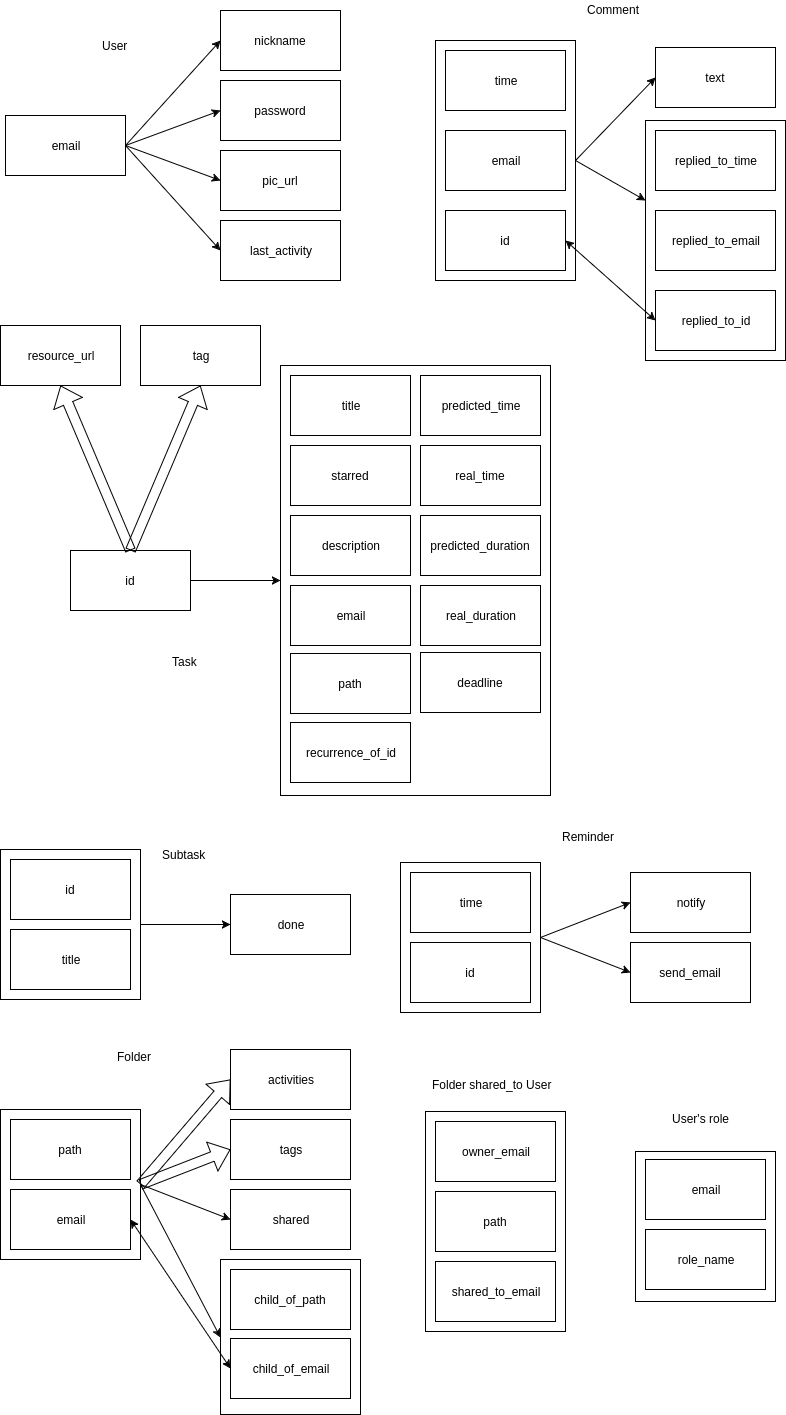
\includegraphics[width = 0.85\textwidth]{Fucntional_Dependancy.png}
  \caption{نمودار وابستگی‌های تابعی اولیه}
  \label{fig:fd1}
\end{figure}

در نهایت نمودار وابستگی‌های تابعی ما به شکل زیر و به فرم نرمال \lr{5NF} خواهد شد:

\begin{figure}[H]
  \centering  
  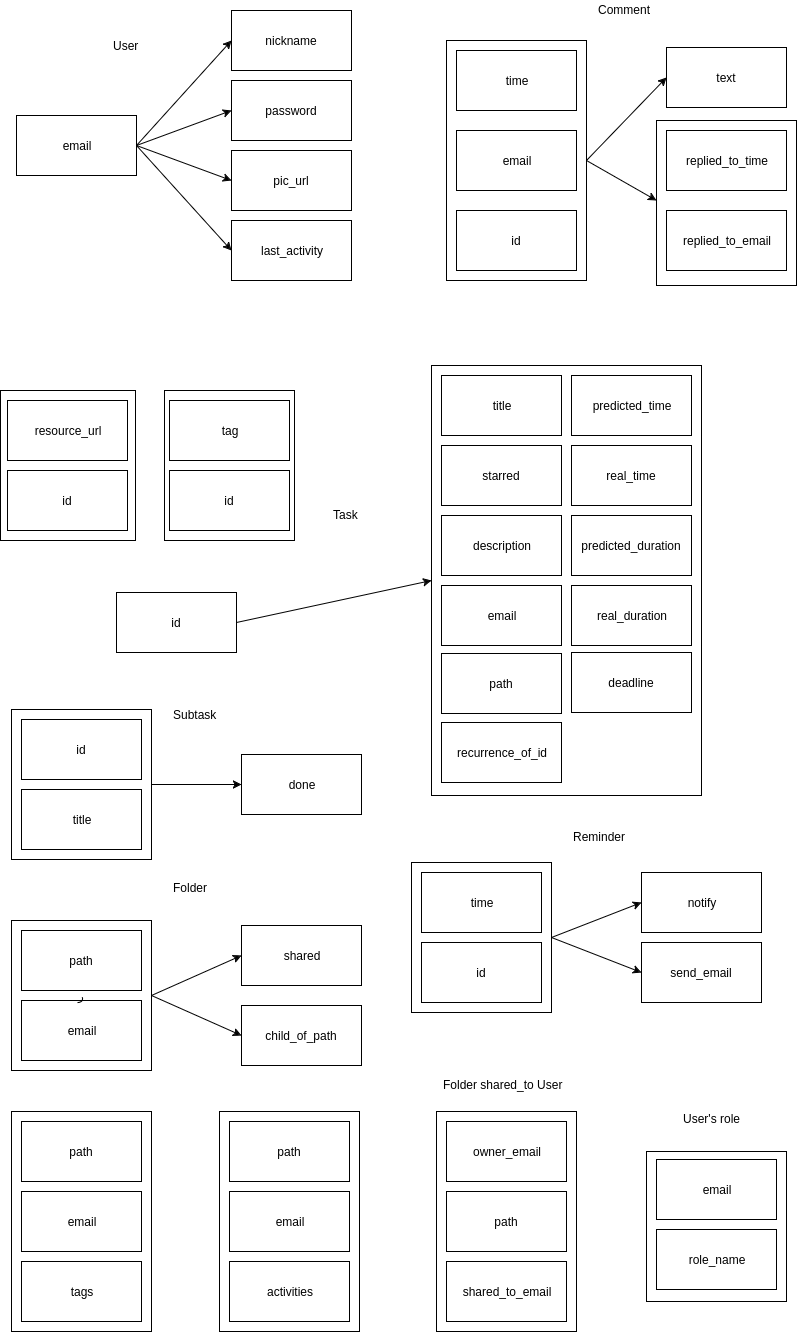
\includegraphics[width = 0.8\textwidth]{Fucntional_Dependancy2.png}
  \caption{نمودار وابستگی‌های تابعی نهایی}
  \label{fig:fd2}
\end{figure}
حتی می‌توان این شما را از این نرمال‌تر هم کرد و به فرم نرمال \lr{6NF} رساند، اما از جایی که همواره مصالحه‌ای بین کارایی و نرمال‌بودن برقرار است دیگر شمایمان را از این نرمال‌تر نمی‌کنیم.
\section*{پیاده‌سازی}
ما برای پیاده سازی از سامانه مدیریت داده postgres استفاده کردیم. برای تعریف رابطه‌ها در این سامانه به صورت زیر عمل کردیم: 

محدودیتهایی که در کلیدها و دامنه‌ها لحاظ نشده‌اند را می‌توان با اظهار یا رهانا پیاده سازی کرد که در در زیر نوشته شده است:

\begin{figure}[hbt!]
  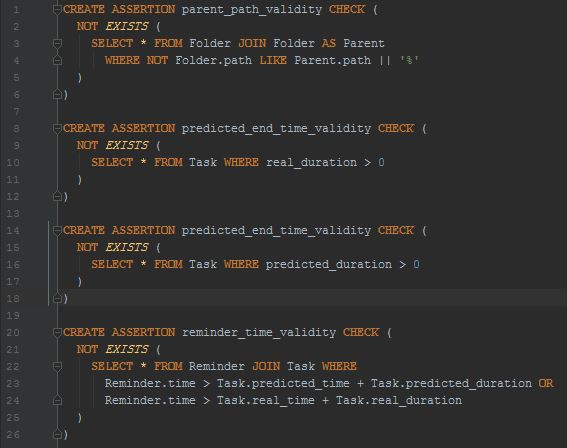
\includegraphics[width =\textwidth]{assertions}
\end{figure}
 همین محدودیتها را می‌توان با رهانا به صورت زیر پیاده سازی کرد:
 
\end{document}